\section{Hardware accelerators}

The rate of complexity in technology doubles approximately every 3.5 months, contrasting with Moore's Law, which historically predicted a doubling of computing capacity every 18-24 months. 
However, in the present era, Moore's Law has slowed down, with computing capacity doubling every 4 years or longer.

The emergence and widespread adoption of deep learning models have ushered in a new era where specialized hardware plays a crucial role in powering a wide range of machine learning solutions. 
Since 2013, the computational requirements for AI training have been doubling every 3.5 months, significantly outpacing the traditional Moore's Law projection of 18-24 months.
To meet the escalating computational demands of deep learning tasks, WSCs are deploying specialized accelerator hardware such as GPUs, TPUs, and FPGAs. 
These accelerators are optimized to handle the intensive processing required for training and inference tasks in deep learning applications.

\subsection{Graphical processing unit}
GPUs have revolutionized data processing by enabling data-parallel computations, where the same program can be executed simultaneously on numerous data elements in parallel. 
This parallelization technique is particularly effective for scientific codes, which are often structured around matrix operations.

Harnessing the power of GPUs typically involves using high-level languages like CUDA and OpenCL. 
Compared to traditional CPU-based processing, GPUs can deliver remarkable speed boosts, sometimes performing computations up to 1000 times faster.

\subsection{Neural networks}
Neural networks are a computational model inspired by the human brain, specifically the perceptron. 
They comprise interconnected nodes, or neurons, organized in layers to process and analyze data. 
Neural networks are utilized to learn data representation, enabling them to learn features and function as classifiers or regressors.

Neural networks have a rich history dating back to the 1940s, with notable developments occurring in the 1980s. 
In recent years, there has been a resurgence of interest in neural networks due to factors such as increased data availability and computational power, with some regarding them as among the top breakthroughs in 2013.

In natural neurons, information is transmitted through chemical mechanisms. 
Dendrites gather charges from synapses, which can be either inhibitory or excitatory. 
Once a threshold is reached, the accumulated charge is released, causing the neuron to fire.
Like its biological counterpart, an artificial neuron receives input signals, which are weighted and summed. 
This sum undergoes an activation function, determining the output signal of the neuron: 
\[h_j(x|w,b)=h_j\left(\sum_{i=1}^{I}w_jx_i-b\right)=h_j\left( \sum_{i=0}^{I}w_ix_i \right)=h_j\left(w^Tx\right)\]
\begin{figure}[H]
    \centering
    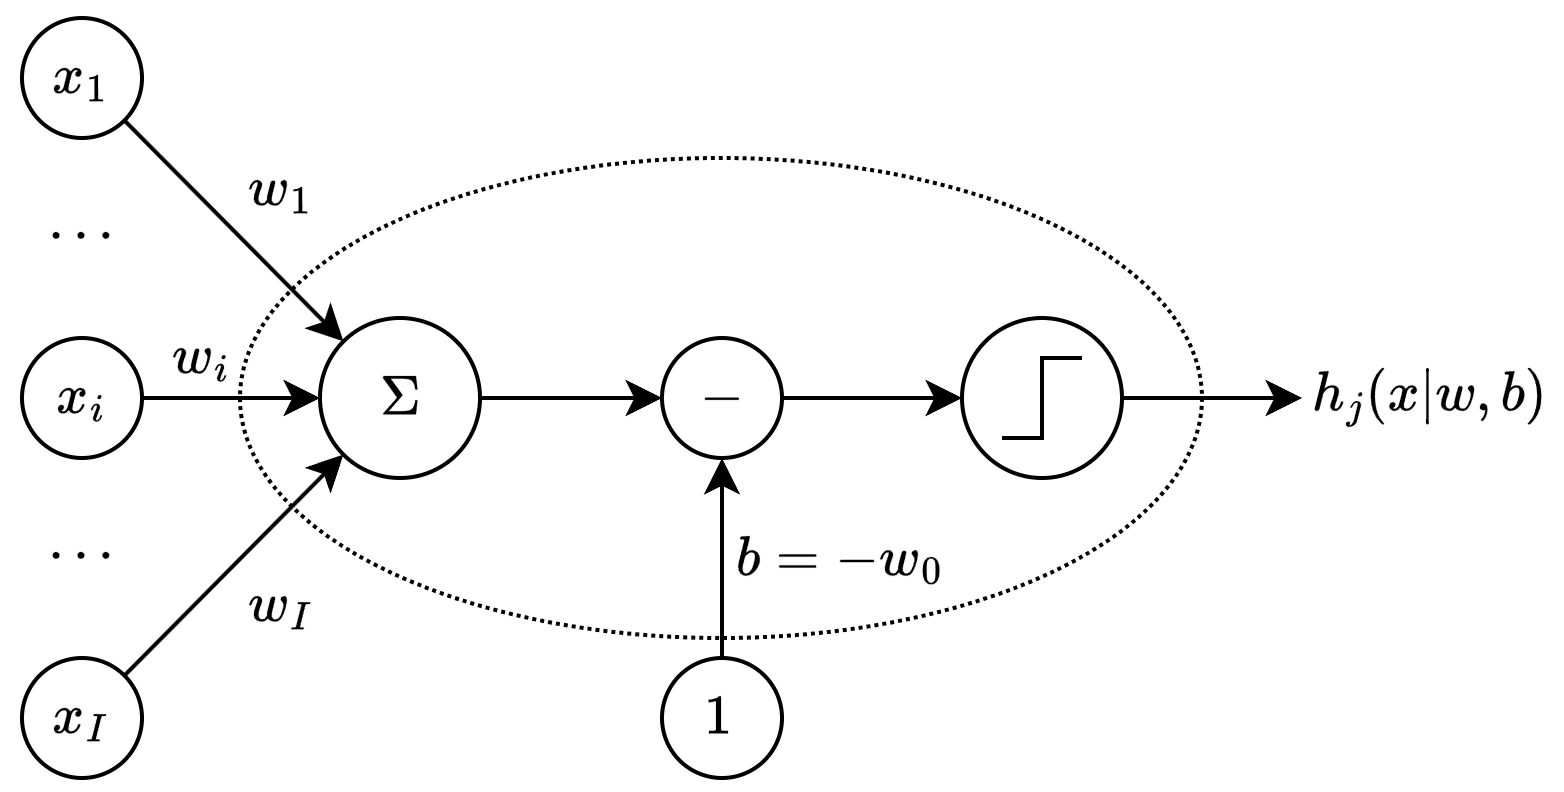
\includegraphics[width=0.5\linewidth]{images/neuron.png}
    \caption{Artificial neuron}
\end{figure}
Neural networks are structured into at least three layers:
\begin{itemize}
    \item \textit{Input layer}: this is where data is initially introduced into the network.
    \item \textit{Hidden layers}: intermediate layers that process and transform the input data.
    \item \textit{Output layers}: the final layer that provides the network's ultimate results or predictions.
\end{itemize}
These layers are interconnected through weighted connections. 
Activation functions, which must be differentiable, determine the output of each neuron. 
Importantly, the output of a neuron is influenced solely by the inputs from the preceding layer.

Neural networks are inherently non-linear models. 
Their behavior is characterized by various factors, including the number of neurons, the choice of activation functions, and the specific values of the weights assigned to connections within the network. 
These factors collectively determine the network's ability to learn and make accurate predictions from the input data.

Learning in neural networks involves several key processes:
\begin{itemize}
    \item \textit{Activation functions}: neurons within the network make decisions based on input data through activation functions.
    \item \textit{Weights}: connections between neurons are adjusted during training, either strengthened or weakened, to optimize performance.
\end{itemize}
Neural networks learn from historical data and examples provided during training. 
This process often involves backpropagation, which utilizes techniques like gradient descent and the chain rule to calculate errors and adjust the model accordingly. 
Errors are evaluated and used to refine the network's parameters, improving its ability to make accurate predictions or classifications. 

Neural networks come in various types, each tailored for specific tasks:
\begin{itemize}
    \item \textit{Feed forward neural network}: standard neural network where information flows in one direction, from input to output.
    \item \textit{Convolutional neural networks} (CNNs): designed for processing grid-like data such as images, with specialized layers for feature extraction and pattern recognition.
    \item \textit{Recurrent neural networks} (RNNs): suitable for sequential data where past information influences the present, often used in natural language processing and time series analysis.
\end{itemize}
These types of neural networks find applications across diverse domains:
\begin{itemize}
    \item \textit{Image recognition}: utilized in technologies like FaceNet and YOLO for tasks such as facial recognition, object detection, and instance segmentation.
    \item \textit{Natural language processing}: leveraged by models like BERT and GPT for applications like chatbots, sentiment analysis, and speech-to-text translation.
\end{itemize}
The potential for innovation and future development in neural networks is extensive. 
With the rapid growth of neural network applications, they are continuously expanding into new and diverse areas such as social media, aerospace, e-commerce, finances, and beyond. 
Additionally, advancements in generative AI are driving innovation in fields like art, music, and content generation, allowing for the creation of novel content through sophisticated generative models.

\paragraph*{Neural networks and GPUs}
GPUs are commonly employed for training neural networks. 
However, the performance of such a synchronous system is constrained by the slowest learner and the slowest messages transmitted through the network. 
As the communication phase is a critical component, a high-performance network is essential for expediting parameter reconciliation across learners.

In configurations involving GPUs, a CPU host is typically connected to a PCIe-attached accelerator tray housing multiple GPUs. 
Within this tray, GPUs are interconnected using high-bandwidth interfaces such as NVlink, facilitating efficient communication and data exchange between the GPUs.

In the A100 GPU, each NVLink lane supports a data rate of $50 \times 4\:Gb/s$ in each direction. 
The total number of NVLink lanes increases from six lanes in the V100 GPU to 12 lanes in the A100 GPU, resulting in a total bandwidth of $600\:GB/s$. 
With the H100 GPU, each GPU can have up to 18 lanes, leading to a total bandwidth of $900\:GB/s$.
\begin{figure}[H]
    \centering
    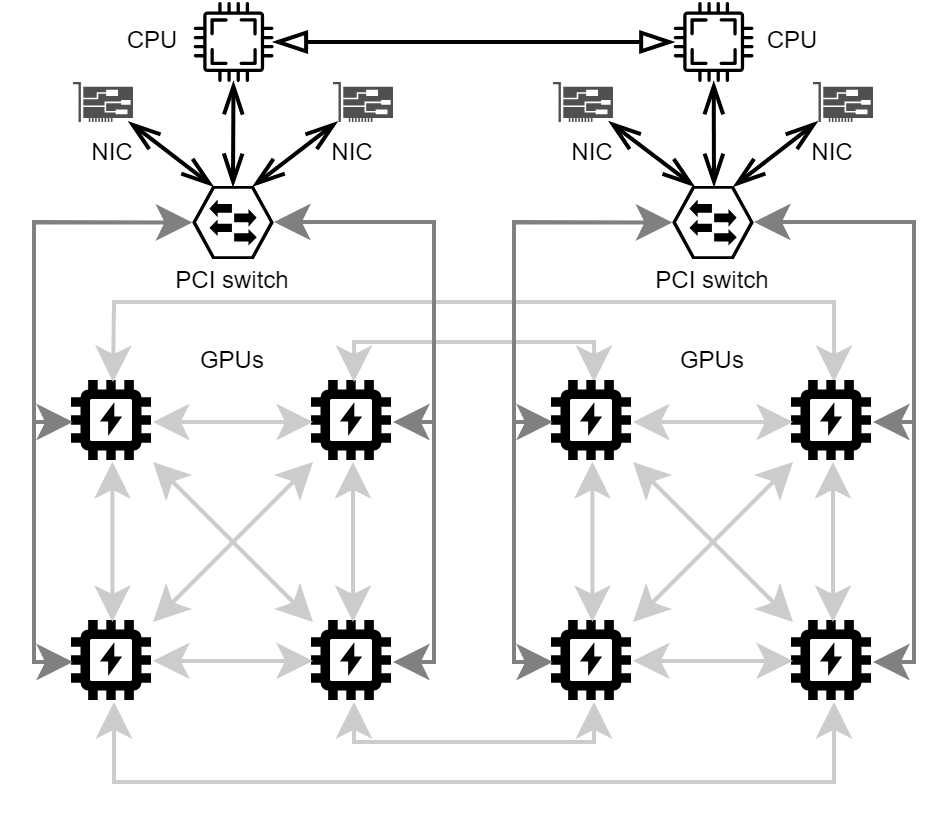
\includegraphics[width=0.75\linewidth]{images/nnt.png}
    \caption{Neural network training}
\end{figure}

\subsection{Tensor processing unit}
Although GPUs are well-suited to machine learning (ML), they are still considered relatively general-purpose devices. 
However, in recent years, designers have increasingly specialized them into ML-specific hardware. 
These custom-built integrated circuits are developed specifically for machine learning tasks and are tailored to frameworks like TensorFlow.

These ML-specific hardware units have been powering Google data centers since 2015, alongside CPUs and GPUs. 
In TensorFlow, the basic unit of operation is a Tensor, which is an n-dimensional matrix.

Tensor Processing Units (TPUs) are extensively used for both training and inference tasks. 
The main versions of Tensor Processing Units are: 
\begin{itemize}
    \item \textit{TPUv1}: inference-focused accelerator connected to the host CPU through PCIe links. 
    \item \textit{TPUv2}: supports both training and inference operations, providing enhanced flexibility and performance.
        In TPUv2, each Tensor Processing Unit (TPU) core consists of an array for matrix computations unit (MXU) and a connection to high bandwidth memory (HBM), which is used to store parameters and intermediate values during computation.
        Specifically, TPUv2 is equipped with 8 GiB of HBM for each TPU core, ensuring ample storage capacity. 
        Additionally, there is one MXU allocated for each TPU core, facilitating efficient matrix computations.
        The hardware layout of TPUv2 comprises 4 chips, with each chip housing 2 cores. 
        This configuration optimizes performance and scalability for machine learning tasks.
        Within a rack, numerous TPUv2 accelerator boards are interconnected via a custom high-bandwidth network, facilitating a collective ML compute power of 11.5 petaflops. 
        This network's high bandwidth capabilities ensure swift parameter reconciliation with precisely controlled tail latencies.
        A TPU Pod, consisting of 64 units, can accommodate up to 512 total TPU cores and $4\:TB$ of total memory. 
        This configuration maximizes both processing power and memory capacity for demanding machine learning tasks.
    \item \textit{TPUv3}: Google's initial venture into liquid-cooled accelerators within their data centers. 
        With a performance boost of 2.5 times compared to its predecessor, TPUv2, this supercomputing-class computational power enables various new ML capabilities such as AutoML and rapid neural architecture search.
        The TPUv3 Pod offers an impressive maximum configuration, boasting 256 devices, totaling 2048 TPU v3 cores. 
        This setup delivers an astounding 100 petaflops of computing power and accommodates 32 TB of TPU memory, ensuring enhanced performance and scalability for demanding machine learning tasks.
    \item \textit{TPUv4}: announced in June 2021, TPUv4 marks the latest advancement in Google's Tensor Processing Unit lineup. 
        Initially deployed to bolster Google's in-house services, TPUv4 is not yet available as a cloud service.
        A single TPUv4 pod comprises 4096 devices, showcasing a remarkable performance increase of approximately 2.7 times compared to its predecessor, TPUv3. 
        With computing capabilities equivalent to around 10 million laptops, TPUv4 sets a new standard for high-performance machine learning hardware.
    \item \textit{TPUv5}: it has two versions (v5e and v5p). 
        The latter one was announced in December 2023 and has been available since early this year.
        Compared to TPUv4, v5p can train large language models like GPT3-175B 2.8 times faster.
        On the other hand, although v5e is slower, it offers more relative performance per dollar compared to v5p.
\end{itemize}
On the other hand, AWS offers Trainium2, specifically optimized for Large Language Models (LLMs). 
Additionally, they provide Graviton4, based on ARM architecture, offering 30\% greater energy efficiency for general AI tasks. 
For AI inference, AWS offers Inferentia2, which boasts 2.3 times higher throughput and up to 70\% lower cost per inference compared to comparable EC2 instances.

\subsection{Field programmable gate array}
FPGAs (Field-Programmable Gate Arrays) are arrays of logic gates that users can program or configure in the field, without relying on the original designers.
These devices consist of carefully designed and interconnected digital subcircuits that efficiently implement common functions, providing extremely high levels of flexibility. 
The individual digital subcircuits within FPGAs are known as configurable logic blocks (CLBs).

VHDL and Verilog are hardware description languages used to describe hardware. 
They enable users to create textual representations of hardware components and their interconnections. 
HDL code resembles a schematic, using text to define components and establish connections between them.

\begin{table}[H]
    \centering
    \begin{tabular}{c|cc}
                  & \textbf{Advantages}                                                                 & \textbf{Disadvantages}                                \\ \hline
    \textit{CPU}  & \makecell{Easily programmable and compatible \\ Rapid design space  \\ Efficiency}  & \makecell{Simple models \\ Small training sets}       \\ \hline
    \textit{GPU}  & \makecell{Parallel execution}                                                       & \makecell{Limited flexibility}                        \\ \hline
    \textit{TPU}  & \makecell{Fast for ML}                                                              & \makecell{Limited flexibility}                        \\ \hline
    \textit{FPGA} & \makecell{High performance \\ Low cost \\ Low power consumption}                    & \makecell{Limited flexibility \\ High-level synthesis}                      
    \end{tabular}
\end{table}